\documentclass{llncs}

\usepackage[utf8]{inputenc}
\usepackage{todonotes}
\usepackage{graphicx}
\usepackage{hyperref}
\usepackage{color}
\usepackage{amsfonts}
\usepackage{amsmath}


\newcommand{\matodo}[1]{\todo[inline, color=green!50]{#1}}
\newcommand{\cetodo}[1]{\todo[inline, color=orange!50]{#1}}

\begin{document}
\title{Running experiments with confidence and sanity}
%
%\titlerunning{Abbreviated paper title}
% If the paper title is too long for the running head, you can set
% an abbreviated paper title here
%
\author{
  Martin Aumüller\inst{1}\orcidID{0000-0002-7212-6476} \and
  Matteo Ceccarello\inst{2}\orcidID{0000-0003-2783-0218}}
%
\authorrunning{M. Aumüller and M. Ceccarello}
% First names are abbreviated in the running head.
% If there are more than two authors, 'et al.' is used.
%
\institute{
  IT University of Copenhagen,
  Denmark\\
  \email{maau@itu.dk}
  \and
  Free University of Bozen, Italy\\
  \email{mceccarello@unibz.it}}
%
\maketitle              % typeset the header of the contribution
%
\begin{abstract}
Analyzing data from large experimental suites is a daily task for
anyone doing experimental algorithmics.
In this paper we report on several approaches we tried for this 
seemingly mundane task, reflecting on the many errors and consequent
mishaps.

We conclude by proposing a workflow, which can be implemented using several
tools, that allows to analyze experimental data with confidence.

\keywords{Experimental algorithmics; Experimental analysis; data analysis}
\end{abstract}

\section{Introduction}

One of the peculiar aspects of \emph{experimental algorithmics}~\cite{DBLP:conf/dimacs/Moret99}
is that the object of the study (an algorithm and its implementation)
is often crafted by the same people carrying out the analysis.
This has the advantage that the insights obtained from preliminary
investigations of early versions of an algorithm can be used to improve the
algorithm itself.
In fact, as also noted by Moret and Shapiro~\cite{DBLP:journals/jucs/MoretS01},
the understanding required for an implementation may uncover features of the
algorithms that would otherwise go unnoticed.
Furthermore, the analysis of experimental results about algorithms can give
insights about aspects that are not easily described by theoretical
models of computation~\cite{DBLP:journals/cacm/McGeoch07}.
At the same time, this feedback-based process leads to the quick
accumulation of obsolete data, referring to old versions of the
algorithms and their implementations.
Not mixing results from different versions of
an algorithm (or implementation) is an obvious requirement, which
however requires some care in practice.
In fact, oftentimes a study involves different algorithms and datasets,
each evolving at a different pace: weeks-old results might be up to date
for one algorithm, and obsolete for another.


As we shall see, the literature is mainly concerned with the design 
and analysis of
experiments, with the communication of the results,
and with reproducibility.
In this paper, instead, we report on our experience with the day to day
tasks that have to be carried out in between those three tasks, and
the approaches we developed to tackle the perils and frustrations of this 
often menial work.

\cetodo{Say that the basic need is to be able to access the experimental
results to run the analysis, basically we need to connect the code running the
experiments with the code carrying out the analysis.}
\cetodo{Mention the rushed publication process, which prompts the need
of not rerunning everything, together with the necessity of saving
money/energy. Therefore we need to have a way of doing this reliably.}
\cetodo{I would like to discuss an \emph{append only} workflow, where
all past results are kept and are easily accessible, since many times
we ask ourselves "I seem to remember that once we got that result".
This is a separate issue from reproducibility, it comes before that.}
\cetodo{We might want to outline a couple of scenarios: investigating
the evolution of the results of some configuration (maybe detecting 
regressions/bugs); debugging, thus finding the change that introduced a
regression, for instance a drop in the recall or speed of the algorithm;
retrieving the most up-to date result for each configuration to do the final
analysis.}


\section{Related work}

Previous works focused mainly on two areas: the design of experiments,
and reproducible research.

Moret and Shapiro~\cite{DBLP:journals/jucs/MoretS01} advocate for the
importance of complementing the theoretical analysis of algorithms
with their implementation.
McGeoch~\cite{DBLP:reference/algo/McGeoch08} gives several guidelines on how to
design and carry out experimental analyses of algorithms.
The book~\cite{DBLP:books/sp/2010BCPP} collects several contributions
on the characterization and analysis of algorithm performance.
Earlier, a Dagstuhl seminar has been devoted to the discussion of the
experimental evaluation of algorithms~\cite{DBLP:conf/dagstuhl/2000ea}.
More recently, a structured approach to the design and evaluation
of experiments has been discussed in~\cite{DBLP:series/ncs/Bartz-BeielsteinP14}.
%
Experimental studies can be influenced by contingent aspects
of the evaluation:
Bartz and Beielstein~\cite{DBLP:reference/sp/Bartz-Beielstein15} discuss
the issue of generalizing the conclusions of experimental studies.
%
McGeoch and Moret~\cite{DBLP:journals/sigact/McGeochM99} and Sanders~\cite{DBLP:conf/dagstuhl/Sanders00}
focus on the reporting of experimental results.

In recent years there has been a discussion about the lack of reproducibility
of research findings in several areas, including 
computer science~\cite{DBLP:journals/cacm/CollbergP16,Hutson725}.
Much effort has been devoted to finding a solution to this issue. Several
contributions have been collected in~\cite{stodden2014implementing} 
and~\cite{kitzes2017practice}.
Among the tools to support reproducible research, 
VisTrails~\cite{DBLP:conf/sigmod/CallahanFSSSV06} allows to
explicitly define reproducible workflows.
\texttt{knitr} and \texttt{Jupyter} take a \emph{literate programming}
approach, allowing experiment's code, analysis, and text to be interleaved
in a single "executable" document.
To solve the issues deriving from software dependencies,
some tools aim at capturing the execution
environment at runtime~\cite{DBLP:journals/cse/Guo12,davison2014sumatra,DBLP:journals/jossw/RampinCSFS16},
while others such as Docker~\cite{DBLP:journals/sigops/Boettiger15}
and Singularity~\cite{kurtzer2017singularity} follow a \emph{declarative}
approach, where the description of the execution environment is part
of the code base


\section{Challenges in running large scale experimental evaluation}



\section{Case study: Engineering a Linear Scan}

As our toy project, we engineer a nearest neighbor search algorithm that just carries out a linear scan over the dataset. 
Formally, we are given a dataset $S \subset \mathbb{R}^d$ of $n$ points in a $d$-dimensional space with a distance measure $\text{dist}\colon \mathbb{R}^d \times \mathbb{R}^d \rightarrow \mathbb{R}$, such that given a query $q \in \mathbb{R}^d$ we want to return a point $p \in S$ that minimizes dist$(p', q)$ over all $p' \in S$.

Solving this problem via a linear scan is a straight-forward exercise in an introduction to programming class: Compare all points $p' \in S$ one by one to $q$, and keep track of the point that is closest to $q$. This results in a running time $O(nd)$ for a single query.

To make this problem more interesting (and introduce more parameters to experiment on), we consider engineering choices to speed up such a linear scan if the distance measure is the inner product $\text{dist}_{\text{IP}}(p,q) = \sum_{1 \leq i \leq d} x_i y_i$, which is analogous to cosine similarity on unit vectors. For the purpose of this project, we consider (i) input representation, (ii) parallelization, and (iii) saving distance computations as factors.

\paragraph{Input representation.}
A vector in $\mathbb{R}^d$ is traditionally represented as $d$ 64-bit floating point values (\texttt{double}). Other engineering choices are 32-bit float (\texttt{float}, or going as far as considering 16-bit representations. Since we guarantee $0 \leq x_i \leq 1$ for normalized vecors, we can use a 16-bit representations of rounded value $\lceil x_i \cdot 256 \rceil / 256$ (which could of course affect the accuracy of the result.)

\paragraph{Parallelization.}
Naïvely, the CPU has to carry out $d$ multiplications and $d-1$ additions to compute the distance of two vectors.
However, we notice that the structure is inherently parallel because the multiplications do not have data dependencies, which is ideal setup for using so-called SIMD instructions (single instruction multiple data). 
In this way, we can split up each vector into blocks of size $B$, and carry out $d/B$ parallel multiplications, $d/B$ parallel additions to aggregate terms in a register of size $B$, and one horizontal sum. 
Depending on the CPU architecture used in the experiment, $B$ is usually 128, 256, or---very recently---512 bits. Moreover, the choice of representing a single vector in $\mathbb{R}^d$ ranges gives a range of possibilities, using 32- or 64-bit floats, or use custom 16-bit representations.

\paragraph{Saving Distance Computations.} Computing the distance 
between two vectors is certainely the most expensive operation in our linear scan. Hence, if we could decide for a data point $p'$ that it probably is not the nearest neighbor looking could increase the performance of our linear scan. We include experiments with a 64-bit sketch using SimHash with probabilistic quality guarantees in our experiments. We review the approach in more detail in Appendix~\ref{app:sketches}.

\medskip

We consider this toy project representable for an experimentation task in a similarity search setting. An individual run is characterized by many different algorithms, there are feedback loops for the engeering choices, one has to handle datasets and their workloads, one has to measure certain attributes of the run, and so on. The experiment has to be carried out on different machines because of the hardware dependencies, which might mean to rent cloud instances to carry out measurements on recent hardware with $B = 512$ bit AVX512 support.

Our code is provided at \url{TODO}. For the scope of this paper, we consider the \emph{support code} that takes care of handling the setup as the main contribution.  

\section{Approaches to experimental evaluation}
After discussing challenges of experimental evaluations and the considered case study, 
we now describe the suggested workflow. 
We split up the discussion into different dimensions of running a successful experimental study. These dimensions are summarized in Figure~\ref{fig:discussion}. 
In the following, each dimension will be introduced with general guidelines and a discussion of our actual solution. 

\begin{figure}
  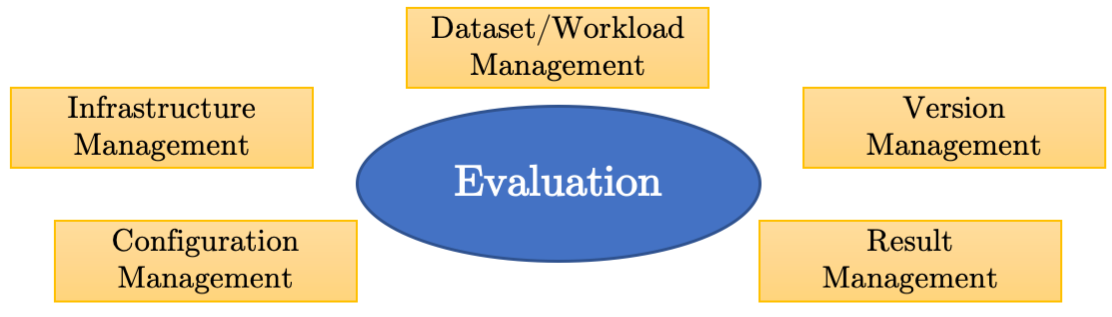
\includegraphics[width=\textwidth]{figs/discussion_points.png}
  \caption{Dimensions for running large-scale experimental evaluations.}
  \label{fig:discussion}
\end{figure}
\subsection{Manage the datasets and workloads efficiently}
\subsection{Manage the experimental configurations clearly}
\subsection{Version everything}
\subsection{Manage the experimental results thoughtfully}
\subsection{Don't repeat yourself}

\section{Conclusions}

\bibliographystyle{alpha}
\bibliography{references}

\appendix

\section{Notes}

There are several challenges when running large experimental suites
for the evaluation of algorithms.

\begin{itemize}
\item Oftentimes the algorithm is modified in response to the results
  of the experimental study. It is important not to mix results from
  different algorithms, and from different code implementations of the
  same algorithm.
\item Usually running the experiments takes a long time, and we don't
  want to re-run all the experiments every time. However, when
  re-using results from old experiments, we need to be sure that we
  are not including undesired and obsolete results.
\item There are two types of experiments: the ones you do during the
  development of the code, which are useful to find out the most
  appropriate parameter ranges, shake out bugs, check assumptions,
  etc; The second kind of experiments is instead devoted to the
  collection of the results of the study. This means that experiments
  are run over a long span of time. It is very important that results
  obtained with different code versions are not mixed.
\item An experiment is run multiple times with the same parameter
  configuration (including the random seed), but only the most recent
  one is interesting.
\item Experiments are run on a machine (or cluster of machines) and then
  analyzed in another.
\item There are \emph{many} experiemnts.
\item The analysis is carried out with different tools (python, R) and
  should run reasonably efficiently
\end{itemize}

Here follows the \emph{keys for a successful experimental evaluation}

\paragraph{Manage the experimental results thoughtfully}

\begin{itemize}
\item Collect everything you need, but nothing more: it's expensive to process too
  much data you don't need
\item Implement a mechanism to keep track of only the latest version of an
  experiment. This is crucial to be able to re-run parameter configurations
  without being worried that some old results are sneaking in. You may also
  need some mechanism to clean up old configurations (and then also some
  mechanism to back up)
\item Keep the analysis efficient (use tools like make)
\item Using a database helps managing changes with database migrations.
\item Maybe: Clear connection between an experimental result and the experimental configuration that ran this experiment?
\end{itemize}

\paragraph{Manage the experimental configurations sanely}

\begin{itemize}
\item Never run experiments from the command line, keep that for testing.
\item Have a file describing all the experiments that will go into the paper. This
  can be:
  \begin{itemize}
  \item A file in a declarative language such as YAML. The pros are that it is
    declarative, the cons are that you have to implement the logic to use it
    anyway.
  \item A simple bash script might be a better option: loops are used to test
      different combinations of parameters, and switch statements are used to
      test experiment groups.
  \item A third alternative is to make the code accept configuration file with all
      the parameters to test. The problem is then that we need to implement the
      logic to handle all these runs, which can be very cumbersome an is
      ultimatly wasted work.
  \end{itemize}
\item All experimental files go into the VCS. 
\item Allow to skip rerunning parameter configurations, so to avoid continuous
  editing of the experimental files. Ideally, you should have a way for your
  code to telle whether an experiment has already been run, giving the option
  to skip runinng it or to "override" the result, actually just appending the
  new result.
 \item Chronological ordering: Use YYMMDD-theme\_of\_experiment as file format.
\end{itemize}

\paragraph{Manage the datasets efficiently}

\begin{itemize}
\item \emph{No manual downloading and preprocessing}. At the very minimum, you want a
  script to download and preprocess your data for you
\item In my experience, `bash` quickly becomes very tangled, and `python` is a mess
  to set up if you have to move on a new machine. Embedding the preprocessing
  (and downloading) code in the experiment's code is the best way to go. You
  get a single development environment to set up, a single entry point for the
  experiments (no need to run a script to preprocess and distribute data as a
  separate step).
\item Maybe the datasets should be versioned?
\item There should be a command to list all available datasets, and remove the ones
  that are no longer needed.
\item Annotate datasets with meta-data necessary in the evaluation (such as workloads and `true' answers to workloads) 
\item Must be possible to create all datasets locally, but those versions should be shared. Can be shared via public http/S3.
\item Always have a small dataset of random data that can be created in a few seconds.
\end{itemize}

\paragraph{The code}

Not just from the point of view of implementation, but maybe even more
prominently from the point of view of usage. That is to say:

\begin{itemize}
\item Keep parameters at the bare minimum. If a parameter never changes across
  experiments, then remove it from the tunable options. That is: keep the
  interface minimal
\item Don't use environment variables. They seem neat and convenient, but they soon
  go out of eyesight and you may forget that some are set to some value. It's
  way better to have all the parameters specified as command line arguments:
  having to repeat them every time is a good reminder to keep the interface
  minimal.
\item Use assertions everywhere, possibly active just during debug. This means that
  you should have a test dataset that can run in a reasonable time in debug
  mode. The problem is that often the problems arise when using large datasets
  that can be handled just in release mode.
\end{itemize}

\paragraph{Provide a Well-Defined Environment}

Your implementation will depend on many different environmental settings such as the libraries needed to run your code and the correct versions of compilers/libraries/OS that you intended to use:
\begin{itemize}
  \item Provide a containerized development environment (nowadays included in programming IDE such as \url{https://code.visualstudio.com/docs/remote/containers}.)
  \item Consider different container formats for running experiments~\cite{arango2017performance}.
  \item Use continuous integration to test all parts of the workflow
\end{itemize}

\paragraph{Version everything}

Keeping the source code under version control might not be sufficient, since
source code revisions (in isolation) lack semantic meaning: you cannot tell
if a version is more recent than another without looking at the VCS DAG.
Furthermore, there are several components that may need versioning in
a project:
\begin{itemize}
  \item Algorithms implementation
  \item The schemas of the database for reporting results (or the fields of 
    the CSV files, if we don't use a database)
  \item Datasets, for which the preprocessing might evolve in time in 
    response to fixing bugs
\end{itemize}
All these components can evolve independently from one another, even within each category
(we can update just one of the many algorithms and datasets under consideration).
These changes should be recorded, but we don't want to re-run all the experiments just because
one dataset was updated. Rather, we would like to re-run only those experiments involving it.
\cetodo{This is rather similar to \texttt{make}, so we keep re-inventing the wheel, 
or the necessities are always the same.}
For this purpose, using the git version of the code is not well suited to this, as it is
shared between all the components.

\section{Review: 1-bit sketches via SimHash}
\label{app:sketches}

\end{document}

